\subsection*{2. Representación Fasorial y Análisis Frecuencial}

\noindent \textbf{2.1)} Dada la señal \( x(t) = 5\cos(2\pi \cdot 1000t + \pi/4) + 3\sin(2\pi \cdot 1500t - \pi/6) \):\par
\bigskip
    \noindent a) Exprese cada componente en forma fasorial.\par
    \bigskip
    
    Para la componente \(5\cos(2\pi \cdot 1000t + \pi/4) \) es:
    \[
    X = 5 \angle \ \pi/4
    \]
    Para la componente \(3\sin(2\pi \cdot 1500t - \pi/6) \) es:\par
    \bigskip
    
    Una señal \(\sin(\omega t + \phi) = \cos(\omega t + \phi - \pi/2)\), entonces su fasor es:
    \[
    X = 3 \angle\ 2\pi/3
    \]
    
    \noindent b) Grafique el diagrama fasorial.\par
    \bigskip

    \begin{figure}[H]
        \centering
        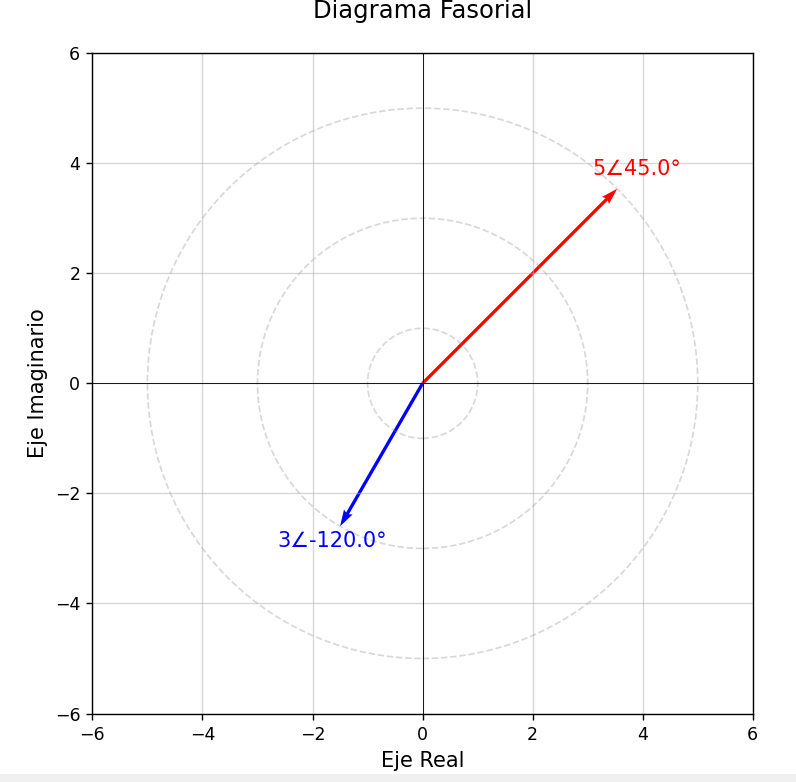
\includegraphics[width=0.5\linewidth]{diagramafasorial_eje2.png}
         \caption{Diagrama Fasorial}
        \label{fig:placeholder}
    \end{figure}

    
    \noindent c) Encuentre la representación exponencial compleja.\par

    \[
x(t)= 5 \ \frac{e^{j(2\pi \cdot 1000 t + \pi/4)} + e^{-j(2\pi \cdot 1000 t + \pi/4)}}{2} +  3 \ \frac{e^{j(2\pi \ 1500 t - \pi/6)} - e^{-j(2\pi \cdot 1500 t - \pi/6)}}{2j}
\]


\noindent \textbf{2.2)} Explique el concepto de fasor rotante y su utilidad en el análisis de señales sinusoidales.\par 
\bigskip

Un fasor rotante es un vector complejo que gira en el plano complejo con velocidad angular proporcional a la frecuencia de la sinusoide $w = 2 \pi f $. Facilita el analísis de señales sinusoidales y de sistemas lineales, ya que convierte senos y cosenos en exponenciales complejas.
